%\usepackage{algorithm}
%\usepackage{algorithmic}

\chapter{PROTOTYPE DESIGN}


\section{Materials and Instruments}
This buffer is designed to be an implement base on current tractor attachments. In this paper, a prototype was developed for designing and experimental purposes. (Figure 5.1) 
\begin{figure}[ht!]
\begin{center}
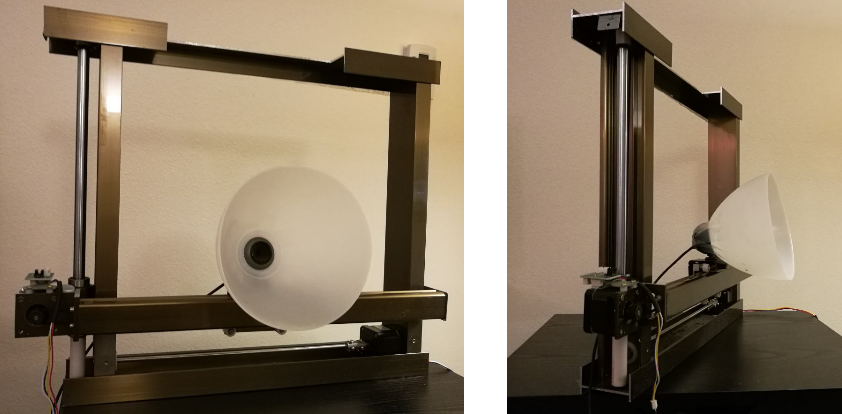
\includegraphics[scale = 0.6]{pics/prototype.png}
\caption{Prototype}
\end{center}
\end{figure}
A camera is installed on the top facing backwards to gather image information. A laser pointer is placed at the end of the row, facing the same direction as the tractor,  and aims at the camera while the tractor moves. Stepper motors are installed on the attachment's frame to offset the attachments, and a Raspberry Pi is used as the central processor to analyze the information gathered by the camera and to give the action commands to the stepper motors. In addition, stepper motor drivers boards are installed to transform the digital control signal to the stepper motors' input. The power supply was designed to use the battery of the tractor, so there is no battery in this prototype. All the parts are listed in Table 5.1.

\begin{table}[ht!]
\begin{center}	
\caption{Parts List}
\begin{tabular}{|l|p{1.5cm}|p{4cm}|l|l|l|}
\hline
Part Name & Vendor & Description  & Unit Cost & Qty. & Sub Total \\ \hline
Camera & Logitech & 480P WEBCAM & - & - & -\\ 
\hline
Stepper Motor & ECOSS INC & Came with frame & - & - &\\ 
\hline
Driver boards & DROK & L298N Motor Drive Controller Board & 6.99 & 1 & 6.99\\
\hline
Microprocessor & CanaKit & Raspberry Pi 2 with Starter Kit & 84.99 & 1 & 84.99\\
\hline
Frames & ECOSS INC & X-Y Stage Table Bed &  169.00 & 1 & 169.00\\
\hline
Wires & Phantom YoYo & 40p Male to Female 40p Female to Female & 4.40 & 1 & 4.40\\
\hline
Camera Hood & - & Lampshade & - & - & -\\
\hline
Curtain & - & Foam Board & - & - & -\\
\hline
Laser Pointer & Fowll & 532 nm Green Laser & 22.99 & 1 & 22.99\\
\hline
Power Supply & Goodwill & Used Charger & 1.99 & 2 & 3.98\\
\hline
Total Cost & & & & & 292.35\\
\hline
\end{tabular}
\end{center}
\end{table}

%对现有农机进行改装,所以成本低。现在实验阶段使用的是,电源,树莓派,摄像头,步进马达,框架,幕布,激光。(做图表,列出成本)

\section{Hardware}

\subsection{Laser Pointer}

A laser pointer is a economic and efficient way to provide a straight and stable reference. Thus, laser guidance is selected to be the guidance system. In order to observe a clear laser reference far in the distance, a high-power laser is the best choice. On the other hand, there are safety problems with laser pointers. High-power laser pointers could damage the retina if they are too close. Based on this safety problem, the laster's power should be restricted. To achieve both low power and far range, a green laser was chosen because, since green light has a shorter wave length than red light, it is able to spread farther than red light with the same power. According to Table 3.2, the maximum eye hazard distance of a 5 $mW$ green laser pointer is only 16 $m$, and the maximum distance from the spot on the screen is over 300 $m$, which is far enough for a row in a crop field. Also the laser pointer can be simply powered by a 3 $V$ lithium battery, which is convenient and inexpensive. According to the above consideration and analysis, a 5 $mW$ green laser was selected.
\begin{table}[ht!]
\begin{center}
\caption{Laser Range}
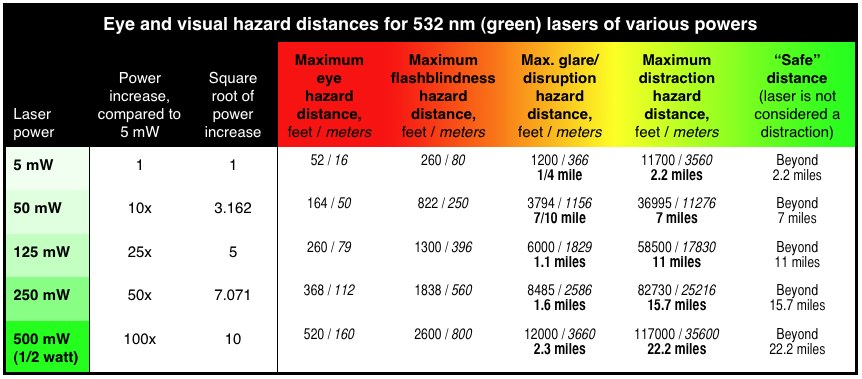
\includegraphics[scale = 0.5]{pics/laserrange.jpg}
\end{center}
\end{table}

\subsection{Buffer Design}


In this built prototype, a lighter and smaller frame was used for convenience. And for the demonstration purpose, no other heavy agricultural attachments will be installed. The camera was mounted on the small sliding block of the frame. Then, a hood was attached on the camera with a curtain covered in front. The hood reduces noise by blocking out light from the angle that the camera does not need to see. The curtain works like a projection screen, so that the laser pointer can leave a spot on it.  A stepper motor is installed on edge of the frame to drive the camera with a belt. The power of the stepper motor along with the control signal was given by a stepper motor driver board. 

The center processor is a Raspberry Pi, which processes the image captured by the camera and then sends the digital control signal to the stepper motor driver board. The wire connections are shown in Figure 5.2.
\begin{figure}[ht!]
\begin{center}
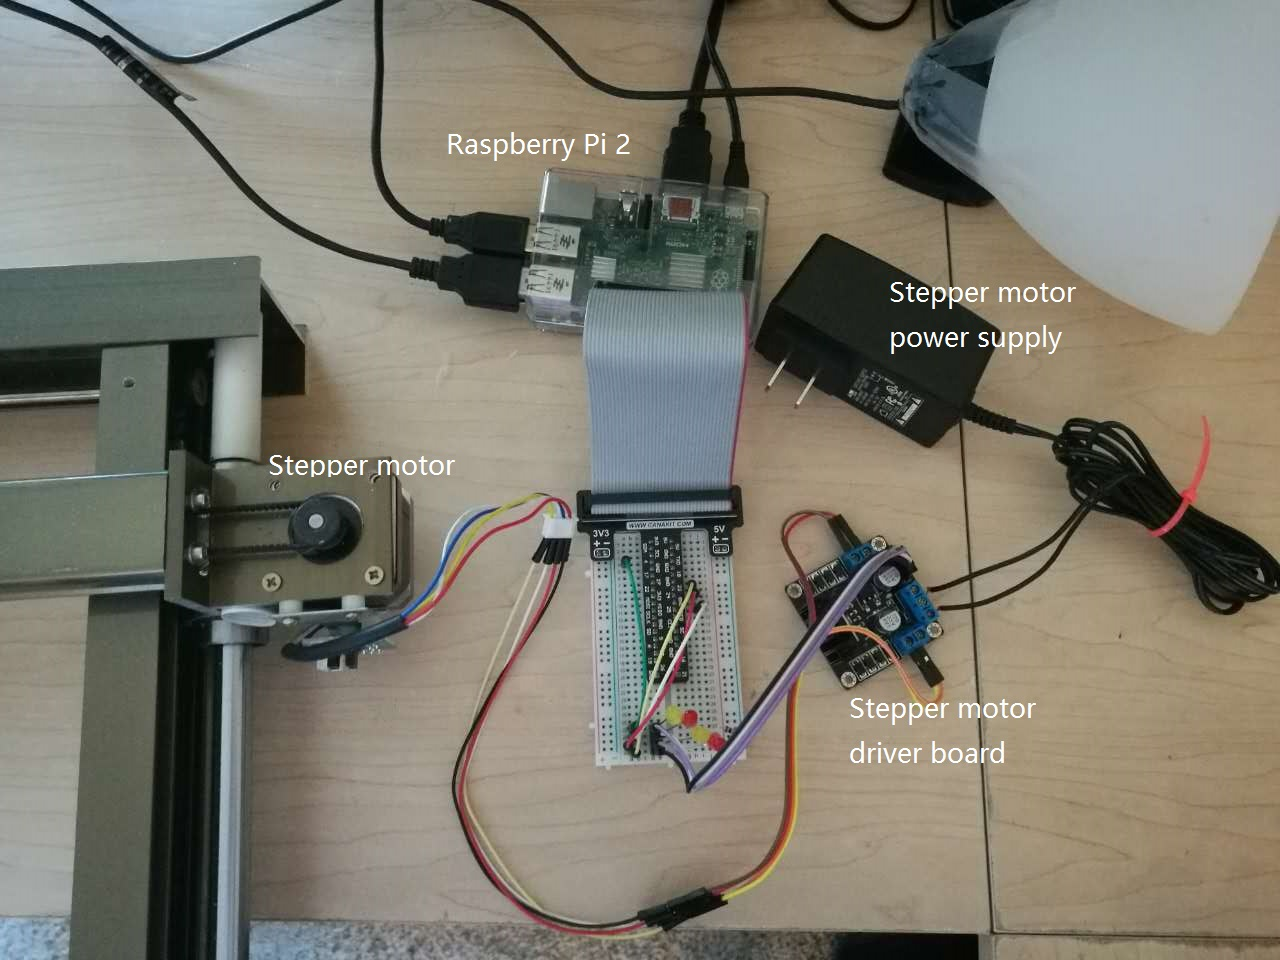
\includegraphics[scale = 0.4]{pics/connection.jpg}
\caption{Wire Connections}
\end{center}
\end{figure}
The prototype works based on the process shown in Figure 4.6. At the beginning, the laser pointer is pointed at the camera curtain. After the origin position is initialized, the frame is moved. The block with the camera, which may have other tractor attachment tools installed, will stay stable.

\section{Software}

\subsection{Image Processing on Raspberry Pi}
The image processing code on the Raspberry Pi was written by following the algorithm of section 4.3.2, with the green color detection based on the HSV color space, and 4.3.3, with the highest light intensity detection. 

Algorithm 1 shows the pseudo-code of green color detection. It blurs the source first to reduce the noise. The next source was converted from RGB color space to HSV color space. Then all the pixels out of the range were masked off, so there is only green color from the source left, which is turned to white. Then the masked image was eroded to minimize the white area. The last step was to find the centroid of the image.

Algorithm 2 works similarly, with two differences. First, the source was converted to GRAY instead of HSV. Second, the pixels other than the pixels that have the highest values were masked off all. 

The highlight detection algorithm dominates at first, and the green color detection algorithm will take over once it generates a steady result.

\begin{algorithm}
\caption{Green Color Detection}
\begin{algorithmic} 
\STATE {$blur(source)$}
\STATE {$green = BGR \rightarrow HSV(source)$}
\FOR {Every pixel of green}
\IF {$60 \leq H \leq 90, 90 \leq S \leq 255, 100 \leq V \leq 255$}
\STATE {$pixel = 255$}
\ELSE 
\STATE {$pixel = 0$}
\ENDIF
\ENDFOR
\STATE {$erode(green)$}
\STATE {$green point = centroid(green)$}				
\end{algorithmic}
\end{algorithm}

\begin{algorithm}
\caption{Highlight Detection}
\begin{algorithmic} 
\STATE {$blur(source)$}
\STATE {$gray = BGR \rightarrow GRAY(source)$}
\STATE {$max$ = max value of all pixel$(gray)$}
\FOR {Every pixel of gray}
\IF {$max-20 \leq pixel \leq max$}
\STATE {$pixel = 255$}
\ELSE 
\STATE {$pixel = 0$}
\ENDIF
\ENDFOR	
\STATE {$erode(gray)$}
\STATE {$highlight point = centroid(gray)$}			
\end{algorithmic}
\end{algorithm}

\subsection{Stepper Motor Control on Raspberry Pi}

%		\begin{table}[ht!]
%			\begin{center}
%				\caption{Raspberry Pi Pins Layout}
%				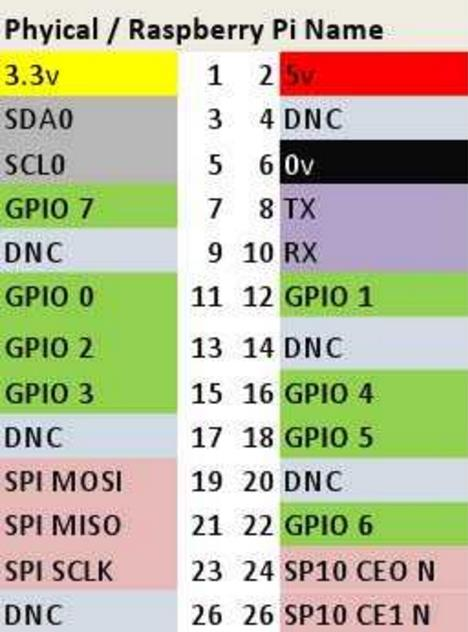
\includegraphics[scale = 0.5]{pipins.jpg}
%			\end{center}
%		\end{table}

%Table 5.3 shows the pins layout of Raspberry Pi. 
$GPIO 0,1,2,3$ is used as the digital signal output. Algorithm 3 is the pseudo-code for motor control. There is a user-defined function called rotate, which enables pin $0,1,2,3$ and initiates the signal sequence at the beginning. Next stepper motor is rotated for one revolution in the clockwise or counterclockwise direction depending on the input. The moving direction is determined by the main function, rotating clockwise if the $x$ coordinate of the point is less than or equal to 310 pixel, rotating counterclockwise if the if the $x$ coordinate of the point is greater than or equal to 330 pixel. There is a 20-pixel window in the middle for NOT MOVING. 

\begin{algorithm}
\caption{Motor Control}
\begin{algorithmic} 
\IF {$point.x \leq 310$}
\STATE {$rotate(clockwise)$}
\ELSIF {$point.x \geq 330$}
\STATE {$rotate(counterclockwise)$}
\ELSE
\STATE {do nothing}
\ENDIF 
%\STATE
\STATE {Function $rotate$($direction$)}
\STATE {$pins = 0, 1, 2, 3$}
\STATE {$sequence[8] = $}
\STATE {$1, 1, 0, 0$}
\STATE {$0, 1, 0, 0$}
\STATE {$0, 1, 1, 0$}
\STATE {$0, 0, 1, 0$}
\STATE {$0, 0, 1, 1$}
\STATE {$0, 0, 0, 1$}
\STATE {$1, 0, 0, 1$}
\STATE {$1, 0, 0, 0$} 
\IF {$direction = clockwise$}
\FOR {$i = 1 \rightarrow 8$}
\STATE {$pins = sequence[i]$}
\ENDFOR
\ENDIF
\IF {$direction = counterclockwise$}
\FOR {$i = 8 \rightarrow 1$}
\STATE {$pins = sequence[i]$}
\ENDFOR
\ENDIF
\end{algorithmic}
\end{algorithm}

\subsection{Multi-thread Programming}
\begin{algorithm}
\caption{Single Thread}
\begin{algorithmic} 
\LOOP
\STATE {Run image processing for one frame}
\IF {$point.x \leq 310$}
\STATE {$direction = clockwise$}
\ELSIF {$point.x \geq 320$}
\STATE {$direction = counterclockwise$}
\ELSE
\STATE {$direction =$ No move}
\ENDIF
\STATE {$rotate(direction)$}
\ENDLOOP		
\end{algorithmic}
\end{algorithm}

Algorithm 4 was the original build for the software part of the laser guidance system; image processing and motor control is in the same loop. It is very inefficient because the clock frequency of the Raspberry Pi CPU is only 900MHz. Since the stepper motor can only rotate one revolution for each loop and the running time for image processing is much greater than motor control, the buffer hardly moves. It may have to rotate for hundreds of revolutions for each result to move to the desired position. 

The CPU of Raspberry Pi is Quad-Core, so it is possible to use multi-thread programming to solve this problem. Algorithm 5 shows the pseudo-code of the multi-thread solution. Image processing and the motor control algorithm run in separate loops in two threads. The parameter $direction$ passes through both threads as a courier and it brings the result from  the image processing part to the motor control part. Therefore, the stepper motor can keep running until the new command comes.

\begin{algorithm}
\caption{Two Threads}
\begin{algorithmic} 
\STATE {Thread 1}
\LOOP 
\STATE {Run image processing for one frame}
\IF {$point.x \leq 310$}
\STATE {$direction = clockwise$}
\ELSIF {$point.x \geq 330$}
\STATE {$direction = counterclockwise$}
\ELSE
\STATE {$direction =$ No move}
\ENDIF
\ENDLOOP	
\STATE {Thread 2}
\LOOP
\STATE {$rotate(direction)$}
\ENDLOOP	
\end{algorithmic}
\end{algorithm}